\begin{song}{title=\predtitle\centering Cestou do Jenkovic \\\large Radůza  \vspace*{-0.3cm}}  %% sem se napíše jméno songu a autor
\begin{centerjustified}
\nejnejvetsi
\sloka 
	^{D}Můj děda z kola ^{Hmi\z }seskočil, ^{C\z }před prázdnou kašnou ^{A}na náměstí.
	
	^{D}Na lavičce chleba ^{Hmi\z }posvačil, ^{C\z }seřídil hodinky ^{A}na zápěstí.

\refren /: ^{D\z}A~čápi z komína ^{A}od cihelny, zobákem ^{C\z }klapou, asi jsou ^{G\z }nesmrtelný. :/

\sloka
	^{D}Tři kluci v bílejch ^{Hmi\z}košilích ^{C\z}dělili se vo ^{A}poslední spartu,

	^{D}ze zídky do záhonu ^{Hmi\z}skočili, ^{C\z}přeběhli ulici a ^{A}zmizeli v parku.

\refren

\sloka
	^{D\z}Ve~voknech svítěj ^{Hmi\z}peřiny, ^{C\z}na bílý kafe ^{A}mlíko se vaří,

	^{D}teď právě začaly ^{Hmi\z}prázdniny, ^{C\z}venku je teplo a ^{A}všechno se daří.

\refren



\end{centerjustified}
\setcounter{Slokočet}{0}
\end{song}


\begin{figure}[h]
\predtitle\centering
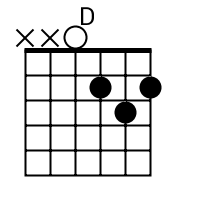
\includegraphics[width=3cm]{../Akordy/d.png}
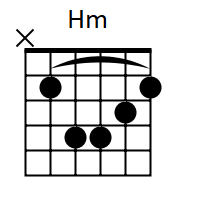
\includegraphics[width=3cm]{../Akordy/hm.png}
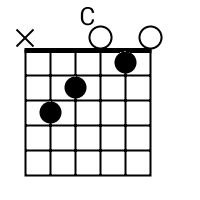
\includegraphics[width=3cm]{../Akordy/c.png}
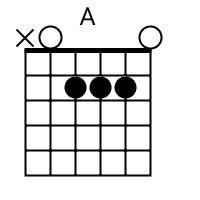
\includegraphics[width=3cm]{../Akordy/a.png}
\end{figure}
